\chapter{Data Encryption in Linux Systems}
\label{chapter:enc-linux}

This chapter explains more detailed the concept of encryption and presents the handling of data encryption in traditional (non-Android) Linux systems.

\section{Encryption explained}
\label{sec:enc-explained}

Encryption is a mathematical transformation takes data requiring protection (plaintext) as input and outputs it into a form not easily understood by unauthorized entities (ciphertext). The ciphertext does not reveal anything about the the original data and its contents.

Encryption can be reversed. This inverse transformation is referred to as decryption. "An encryption process has a corresponding decryption process, which is used to reverse the encrypted data (ciphertext) back to its original content (plaintext)\cite{enc-basics}."

Both the encryption and decryption process use a cryptographic key which is a string of binary digits.

\begin{figure}[h]
\centering
\begin{minipage}{0.45\textwidth}
\centering
  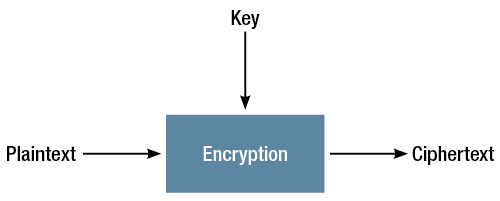
\includegraphics[width=.9\linewidth]{src/img/encrypt/plain2cipher.jpg}
  \caption{Encryption\cite{enc-basics}}
  \label{fig:encrypt-fig}
\end{minipage}\hfill
\begin{minipage}{0.45\textwidth}
\centering
  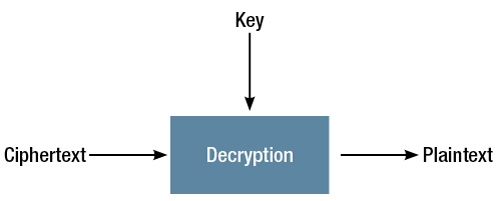
\includegraphics[width=.9\linewidth]{src/img/encrypt/cipher2plain.jpg}
  \caption{Decrpytion\cite{enc-basics}}
  \label{fig:decrypt-fig}
\end{minipage}
\end{figure}

In the case of disk encryption, each blockdevice or individual file (depending on encryption type) is split into equal chunks called sectors. The encryption operations are then done on a per-sector basis. Therefore, there is a 1 to 1 correspondence between the encrypted sectors and the original data.

Whenever a fragment of data from the blockdevice/file is necessary, the whole sector (or sectors) that contains the data will be read from disk, decrypted and temporarily stored in memory.

Similarly, each write operation results in all sectors containing the data being re-encrypted completely.

The cryptographic key corresponding to a blockdevice/file, called \textit{master key}, needs to be supplied every time the respective device is to be mounted.

The following are some of the possible methods of storing and cryptographically securing a master key with a keyfile\cite{disk-enc}:
\begin{enumerate}
\item \textbf{Stored in a plaintext keyfile}

The master key is stored in a file in readable form. The file, called a \textit{keyfile}, can be placed on a removable device that is only connected to the computer when mounting the encrypted parts of the disk.

\item \textbf{Randomly generated on-the-fly for each session}

In cases like swap space or a /tmp encryption, it is not necessary to keep a persistent master key. Instead, a new key can be randomly generated for each session. This means that once unmounted, all files written to the partition in question can never be decrypted again.

\item \textbf{Stored in passphrase-protected form in a keyfile or on the disk itself}

The master key can be protected with a secret passphrase, which will need to be entered each time the encrypted block device or folder is mounted.
It is usually not used for de/encrypting the disk data directly, though. For example, in the case of stacked filesystem encryption, each file can be automatically assigned its own encryption key. Whenever the file is to be read/modified, this file key first needs to be decrypted using the main key, before it can itself be used to de/encrypt the file contents.

\end{enumerate}

\subsection{Benefits of disk encryption}
\label{sub-sec:benefits-enc}

Disk encryption is the process of storing data on disk in an encrypted form. The files only become available in readable form while the system is running and unlocked with the corresponding key.

Disk encryption methods aim to provide three distinct properties:
\begin{enumerate}
\item The data on the disk should remain confidential
\item Read and write operations should both be fast, regardless of where on the disk the data is stored
\item The overhead introduced by the encryption method should not be kept to a minimum (i.e., the amount of storage used for encrypted data should not be significantly larger than the size of plaintext)
\end{enumerate}

Disk encryption can prevent unauthorized reading of the data when the disk is
\cite{disk-enc}:
\begin{itemize}
\item in a place where unauthorized people might gain access while unsupervised
\item lost or stolen
\item in the repair shop
\item discarded after its end-of-life
\end{itemize}

The system will still be vulnerable to
\cite{disk-enc}:
\begin{itemize}
\item Attackers who can break into the system while it is running and after the encrypted parts of the disk have already been unlocked and mounted.
\item Attackers who are able to gain physical access to the computer while it is running or very shortly after it was running.
\item A government entity which may obtain your keys/passphrases using various techniques of coercion.
\end{itemize}

\subsection{Data Encryption vs System Encryption}
\label{sub-sec:de-vs-se}

\textbf{Data encryption} is defined as encrypting only the user's data itself (usually stored in the \texttt{/home} directory). While it is the simplest and least intrusive type of disk encryption, it has some significant drawbacks. The main problem is that data may be accessible trough the swap partition or temporary files created by some processes, both of which are not encrypted.

\textbf{System encryption} is the encryption of the operating system and user data, which helps to address some of the inadequacies of data encryption. It prevents unauthorized physical access to data, regardless of where inside the system it is stored. However, decryption must take place at boot time, in order for the system to be able to start.

"In practice, there is not always a clear line between data encryption and system encryption\cite{disk-enc}."

Finally, it is important that disk encryption be viewed as an addition to the existing security mechanisms of the operating system.

\subsection{Block Encryption vs Stacked File System Encryption}
\label{sub-sec:be-vs-sfse}

The two approaches to disk encryption are block-based and file-based. Block encryption means that the actual encryption process happens when the filesystem writes a block of data on the disk. Its advantages are simplicity and transparency. However, the method lacks granularity, i.e., treating each file differently. This is the type of encryption used in Android 3.0 and later.

A more detailed comparison of block-based encryption and file-based encryption is presented in the table in the eCryptfs frequently asked questions section\footnote{\url{http://ksouedu.com/doc/ecryptfs-utils/ecryptfs-faq.html\#compare}}.

\section{eCryptfs}
\label{sec:de-ecryptfs}

As mentioned before, eCryptfs is a stacked file system which manages data encryption. Now, details about it and the advantages and disadvantages is brings will be presented.

Originally authored by Michael Halcrow and the IBM Linux Technology Center, eCryptfs is derived from Erez Zadok's Cryptfs, and the FiST framework for stacked filesystems. eCryptfs extended Cryptfs to provide advanced key management and policy features\cite{ecryptfs-paper}.

It has already been mentioned that eCryptfs uses a randomly generated File Encyption Key(FEK) for each file and that this key is also encrypted. Also noteworthy is that the FEK in its encrypted form is actually stored together with the encrypted file. This adds the possibility of transferring a file while encrypted with the ability to gain access with the proper credentials.

\subsection{Architecture}
\label{sub-sec:arch-ecryptfs}

eCryptfs is implemented mainly as a kernel module. It uses a number of userspace utilities to perform key management functions.

\fig[scale=0.24]{src/img/ecryptfs/arch.png}{img:ecryptfs-arch}{eCryptfs Architecture\cite{ecryptfs-paper}}

The kernel module encrypts the file contents using the kernel cryptographic API. A keystore component extracts the header information from individual files while a callout application evaluates the header information against the target policy and performs the corresponding operations.

Key management is done in userspace for two main reasons. The first is to reduce the complexity of the code running in kernelspace. The second is due to the fact that management operation are only required when opening/closing a file. Since these operations are relatively infrequent, the overhead does not constitute an issue.

\subsection{Cryptographic Operations}
\label{sub-sec:crypt-ops-ecryptfs}

Most of the data encryption is done in the kernel module, and hence eCryptfs makes use of the kernel cryptographic API to perform the encryption and the decryption operations. One of the primary motivators in implementing eCryptfs in the kernel is to avoid the overhead of context switches between userspace and kernel space, which is frequent when dealing with pages in file I/O.

The underlying file format for eCryptfs is based on the OpenPGP format described in RFC2440\cite{rfc}.

\begin{figure}[h!]
\centering
    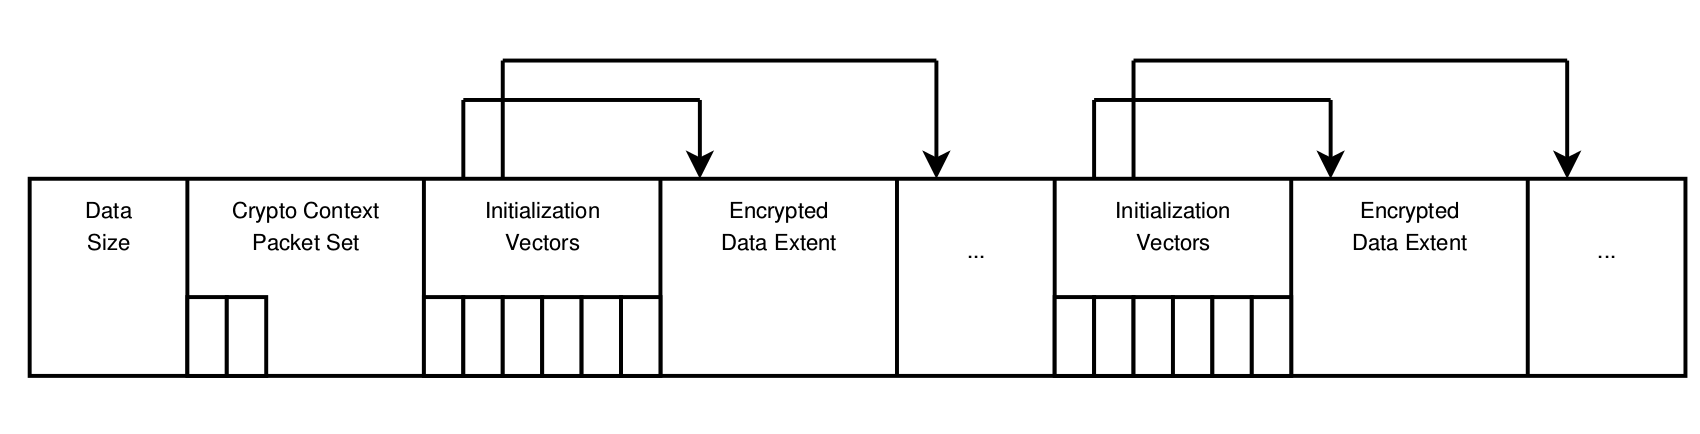
\includegraphics[width=0.92\textwidth]{src/img/ecryptfs/fileformat.png}
\caption{eCryptfs File Format\cite{ecryptfs-paper}}
\end{figure}

An aspect where eCryptfs deviates from the standard is the introduction of \textit{data extents}. This is done in order to accommodate random access while maintaining performance. The OpenPGP standard assumes that the encryption and decryption is done as an atomic operation over the entire data contents of the file; there is no concept of a partially encrypted or decrypted file. The data is encrypted using what is known as a chained block cipher(CBC\abbrev{CBC}{Chained Block Cipher}). This means that each block of plaintext, with the exception of the first, is combined with the previous block ciphertext through a XOR operation before being encrpyted. Evidently, the same process must be followed when decrypting. Thus, reading a byte from a file requires decrypting all leading bytes. Conversely, writing a byte incurs encrypting all trailing bytes from that file. For large files, reading a byte towards the end of the file or writing a byte at the beginning of it would be inefficient.

Using extents, each part of a file is encrypted separately; reading or writing a byte requires operations only on the extent containing the respective byte. An extent containing initialization vectors(IV\abbrev{IV}{Initialization Vector}) precedes a group of extents which used the respective IV's (each extent has an unique IV). These initialization vectors are used to XOR the first block of data when encrypting/decrypting.

Another challenge is treating \textit{sparse files}. A sparse file is a file that contains regions where no data is written, also known as \textit{holes}. The file system normally uses special markers for these regions and sets the filesize in accordance. Thus, less space on the disk is used to store the file. When reading from these regions, the file system simply fills in with zero's.

Although eCryptfs could use markers, e.g. IV's consisting of all zero's, to implement a similar behaviour, this may constitute a breach in security, since it becomes readily apparent to a potential attacker which regions are sparse.
Therefore, eCryptfs prefers to relegate how to treat sparse files to something policy decides.

\subsection{Key Management}
\label{sub-sec:keys-ecryptfs}

eCryptfs aims to operate transparently. The fact that files are encrypted should not be a concern to the user.

Every file is encrypted with a randomly generated session key. This session key is stored in the cryptographic metadata for the file. When a newly created file is closed, the session key is encrypted once for each authentication token associated with the file and then written in the file header. When the file is opened, the encrypted keys are read from the header and an authentication token corresponding to the file. If not found, an action in accordance with the active policy is taken.

"Passphrase authentication tokens in eCryptfs exist in three forms: non-passphrased, saltless, and salted\cite{ecryptfs-paper}." To minimise the vulnerability against a passphrase dictionary attack, a salt value is concatenated with the passphrase and the result is iteratively hashed. The result of the hashing operation constitutes the identifying signature for the authentication token.

The key callout application is the primary connection between the eCryptfs kernel module and the userspace key management code. Depending on the policy and the file in question, it may make calls through the PKI API or it may search for a salted passphrase with a particular signature. The eCryptfs daemon listens to a socket and whenever policy requires that the user be prompted for a passphrase, the callout application can use the socket to request the daemon to prompt the user and then get the result back.

\subsection{Encrypting a Directory Using eCryptfs}
\label{sub-sec:encrypt-dir-ecryptfs}

This is an example of how to encrypt a user directory. It relies on the \textit{ecryptfs-utils} package being installed. Although the operations can be performed manually, for the purpose of this example there is no need to go into such amount of detail. More details on the Arch Linux page on eCryptfs\cite{ecryptfs}.

The name \texttt{secret} will be used for the created directory.

Firt step is to create the required directories:
\begin{lstlisting}[numbers=none]
$ mkdir ~/.secret ~/secret ~/.ecryptfs
$ touch ~/.ecryptfs/secret.conf ~/.ecryptfs/secret.sig
\end{lstlisting}

The encrypted data will be stored in the \texttt{\textasciitilde/.secret} directory.
\texttt{\textasciitilde/secret} is the location where the \texttt{\textasciitilde/.secret} will be mounted as an eCryptfs file system.

Next, the full paths must be added to \texttt{\textasciitilde/.ecryptfs/secret.conf}. They will be used later to mount/unmount data.
\begin{lstlisting}[numbers=none]
$ echo "/home/$USER/.secret /home/$USER/secret ecryptfs" > ~/.ecryptfs/secret.conf
\end{lstlisting}
Note that \texttt{\$USER} should be expanded by the shell to the current username.

A mount passphrase must be added to the keyring:
\begin{lstlisting}[numbers=none]
$ ecryptfs-add-passphrase
Passphrase: 
Inserted auth tok with sig [78c6f0645fe62da0] into the user session keyring
\end{lstlisting}

The ouput signature is added to \texttt{\textasciitilde/.ecryptfs/secret.sig}
\begin{lstlisting}[numbers=none]
$ echo 78c6f0645fe62da0 > ~/.ecryptfs/secret.sig
\end{lstlisting}

Optionally, a passphrase for filename encryption can be appended to the same file
\begin{lstlisting}[numbers=none]
$ ecryptfs-add-passphrase
Passphrase: 
Inserted auth tok with sig [326a6d3e2a5d444a] into the user session keyring
 $ echo 326a6d3e2a5d444a >> ~/.ecryptfs/secret.sig
\end{lstlisting}

To mount \texttt{\textasciitilde/.secret} on \texttt{\textasciitilde/secret}:
\begin{lstlisting}[numbers=none]
$ mount.ecryptfs_private secret
\end{lstlisting}
The mount options are automatically generated using the information stored in \texttt{secret.conf} and \texttt{secret.sig}.

Similarly, to unmount:
\begin{lstlisting}[numbers=none]
$ umount.ecryptfs_private secret
\end{lstlisting}
